\documentclass[a4j,12pt]{jarticle}


% \usepackage{a4j}
\usepackage{fancyhdr}
\usepackage{lastpage}

% \usepackage{showkeys}
% \usepackage[dvips]{graphicx}

\usepackage{bm}

\usepackage{amsmath}
\usepackage{amsfonts}
\usepackage{amssymb}
\usepackage{slashed}
% \usepackage{mathbbol}  % 数字も白抜きにしてくれる
\usepackage{multirow}  % Tableで複数のセルにまたがるセルを作れる

\usepackage[a4paper,top=2.5cm,bottom=2.5cm,left=2.5cm,right=2.5cm,headsep=10pt]{geometry}
% \usepackage{graphicx}           % tikzで使う graphicxと競合するので排除
% \usepackage[usenames]{color}
% \usepackage[usenames,dvipdfmx]{color}    % optionは同時に指定出来る。
\usepackage[dvipsnames,dvipdfmx]{xcolor}    % optionは同時に指定出来る。


\usepackage[british]{babel}
\input{colordvi.tex}

\usepackage[dvipdfm,colorlinks,pagebackref,pdfusetitle,urlcolor=blue,citecolor=MidnightBlue,linkcolor=MidnightBlue,bookmarksnumbered,plainpages=false]{hyperref}



\input{dummy.tex}

%%% tikzセッティング %%%%%%%%%%%%%%%%%%%%%%%%%%%%%%%
\usepackage[dvipdfmx]{graphicx}
\usepackage{tikz}
\usetikzlibrary{arrows,shapes,patterns,snakes,calc}
\input{arrowsnew}
\usetikzlibrary{decorations.markings}
\usetikzlibrary{positioning}
%%% end of tikz %%%%%%%%%%%%%%%%%%%%%%%%%%%%%%%%%%%%

\usepackage[hang,bf,figurename=Fig.\ , tablename=Table\ ,margin=1cm]{caption}
\renewcommand{\captionfont}{\footnotesize}

%%% listingsセッティング %%%%%%%%%%%%%%%%%%%%%%%%%%%
\usepackage{listings, jlisting}
\renewcommand{\lstlistingname}{Code}
\definecolor{mygreen}{rgb}{0,0.6,0}
\definecolor{mygray}{rgb}{0.5,0.5,0.5}
\definecolor{mymauve}{rgb}{0.58,0,0.82}

\lstset{ %
  % language=Octave,                 % the language of the code
  backgroundcolor=\color{white},   % choose the background color; you must add \usepackage{color} or \usepackage{xcolor}
  basicstyle=\footnotesize,        % the size of the fonts that are used for the code
  breakatwhitespace=false,         % sets if automatic breaks should only happen at whitespace
  breaklines=true,                 % sets automatic line breaking
  captionpos=t,                    % sets the caption-position to bottom
  commentstyle=\color{mygreen},    % comment style
  deletekeywords={...},            % if you want to delete keywords from the given language
  escapeinside={\%*}{*)},          % if you want to add LaTeX within your code
  extendedchars=true,              % lets you use non-ASCII characters; for 8-bits encodings only, does not work with UTF-8
  frame=single,                    % adds a frame around the code
  keepspaces=true,                 % keeps spaces in text, useful for keeping indentation of code (possibly needs columns=flexible)
  keywordstyle=\color{blue},       % keyword style
  morekeywords={*,...},            % if you want to add more keywords to the set
  numbers=left,                    % where to put the line-numbers; possible values are (none, left, right)
  numbersep=5pt,                   % how far the line-numbers are from the code
  numberstyle=\tiny\color{mygray}, % the style that is used for the line-numbers
  rulecolor=\color{black},         % if not set, the frame-color may be changed on line-breaks within not-black text (e.g. comments (green here))
  showspaces=false,                % show spaces everywhere adding particular underscores; it overrides 'showstringspaces'
  showstringspaces=false,          % underline spaces within strings only
  showtabs=false,                  % show tabs within strings adding particular underscores
  stepnumber=1,                    % the step between two line-numbers. If it's 1, each line will be numbered
  stringstyle=\color{mymauve},     % string literal style
  tabsize=2,                       % sets default tabsize to 2 spaces
  title=\lstname                   % show the filename of files included with \lstinputlisting; also try caption instead of title
}
%%% ned of listings セッティング %%%%%%%%%%%%%%%%%%%%%%%%%%%


\pdfstringdefDisableCommands{%
    \renewcommand*{\bm}[1]{#1}%
    % any other necessary redefinitions 
}

%%%今村セッテッティング%%%%%%%%%%%%%%%%%%%%%%%%%%%%%
\newcommand{\CC}{\mathbb{C}}
\newcommand{\ZZ}{\mathbb{Z}}
\newcommand{\RR}{\mathbb{R}}
\newcommand{\HH}{\mathbb{H}}

\newcommand{\hf}{\frac{1}{2}}
\newcommand{\tr}{{\rm tr}}
\newcommand{\ind}{{\rm ind}}
\newcommand{\ol}{\overline}
\newcommand{\ul}{\underline}
\newcommand{\up}{\uparrow}
\newcommand{\dn}{\downarrow}
\newcommand{\wt}{\widetilde}
\newcommand{\ra}{\rightarrow}
\newcommand{\wh}{\widehat}


%%%横山セッティング%%%%%%%%%%%%%%%%%%%%%%%%%%%%%%%%%
\newcommand{\NN}{\mathcal{N}\!}
\newcommand{\DD}{\mathcal{D}}
\newcommand{\UU}{U(1)}
\newcommand{\dd}{\mathrm{d}}
\renewcommand{\SS}{\mathbf{S}}
\renewcommand{\Im}{\mathrm{Im}}
\renewcommand{\Re}{\mathrm{Re}}
\renewcommand{\<}{\langle}
\renewcommand{\>}{\rangle}
\newcommand{\Tr}{{\rm Tr}}

\renewcommand{\r}{\mathrm}

\newcommand{\sign}{\mathrm{sign}}

\newcommand{\lra}{\leftrightarrow}
\newcommand{\LL}{\mathcal{L}}
\newcommand{\la}{\leftarrow}
\newcommand{\ro}{\sqrt}
\newcommand{\Ra}{\Rightarrow}
\newcommand{\Pexp}{\mathrm{Pexp}}

\newcommand{\nn}{\nonumber \\}
\newcommand{\1}{\mbox{1}\hspace{-0.25em}\mbox{l}}

%数字のみ対応
\newcommand{\Maru}[1]{\ooalign{
\ifnum#1<10 \hfil\resizebox{.9\width}{.85\height}{#1}\hfil
\else
\hfil\resizebox{.6\width}{.8\height}{#1}\hfil
\fi
\crcr
\raise.1ex\hbox{$\bigcirc$}}}

%全文字対応
\newcommand{\maru}[1]{\ooalign{
\hfil\resizebox{.8\width}{\height}{#1}\hfil
\crcr
\raise.1ex\hbox{\large$\bigcirc$}}}


\newcommand{\nord}[1]{\vcentcolon\mathrel{#1}\vcentcolon}
\providecommand{\vcentcolon}{\mathrel{\mathop{:}}}


\def\P{\mathop{\cal P}}
\def\diag{\mathop{\rm diag}}


\def\Re{\mathop{\rm Re}\nolimits}
\def\Im{\mathop{\rm Im}\nolimits}
\def\Det{\mathop{\rm Det}\nolimits}
\def\sign{\mathop{\rm sign}\nolimits}


%%% rap %%% - make two letters overlap
\newcommand{\rap}[2]
{\setbox1=\hbox{#1}%
\setbox2=\hbox to\wd1{\hss #2\hss}%
\mbox{\rlap{\box1}\box2}}

%\newcommand{\sla}[1]{\rap{$#1$}{/}}
\newcommand{\sla}[1]{\rap{$#1$}{$\backslash$}}


\def\DY#1{{\MyGreen [DY: #1]}}
\newcommand{\MyGreen}{\color [rgb]{0,0.7,0}}

\usepackage[vcentermath]{youngtab}
% \Yboxdim4pt
\newcommand{\Y}{\yng}
\newcommand{\Young}{}


%%%title def%%%%%%%%%%%%%%%%%%%%%%%%%%%%%%%%%%%%%%%%%%%%%%%

\makeatletter
\def\maketitle{
\noindent
{\Large \@title \par\vskip 2pt}
\noindent
{\large \@date \hspace{4pt} \@author}
%\\[-2pt]
%\noindent------------------------------------------------------------------------------------------
\par\vskip 1.5em
}

\author{横山 大輔}
\date{\today}
%%%本文%%%%%%%%%%%%%%%%%%%%%%%%%%%%%%%%%%%%%%%%%%%%%%%%%%%%%%%%

% \title{\centerline{Lecture 2}}
\begin{document}
% \maketitle
% \begin{abstract}

% \end{abstract}
% \tableofcontents

  \pagestyle{fancy}
  \renewcommand{\headrulewidth}{0.0pt}
  \rhead{}
  \lhead{}
  \cfoot{[\ \scshape\oldstylenums{\thepage}\ / %
    \scshape\oldstylenums{\pageref{lastpage}} ]}
%  \rfoot{\@author}

% \setcounter{section}{}
% \setcounter{subsection}{}
% \setcounter{subsubsection}{}

\centerline{\Large \bf  Lecture 10}

% \vspace{12pt}
% \DY{なにかコメント}

% \vspace{-12pt}




\section{Type I superstring theory}

What we will learn:
\vspace{-4pt}
\begin{itemize}
 \setlength{\itemsep}{0pt}
 \item Type I superstring theory.
 \item In type I theory, we only have D$1$-, D$5$-, and D$9$-, branes.
 \item O$9^-$-plane is needed for type I to be consistent theory.
 \item T-duality of type I theory.
\end{itemize}
\vspace{-4pt}


So far, we have learnt two kinds of superstring theory, which are type IIA and IIB.
Both of them are closed superstring theory.
Note that we also learnt about D-branes in type II theories, which leads open string.
However, note that we are considering a situation in which there exist D-branes,
so it is not a theory.


Actually, an open string cannot exist in type II theories (without D-branes),
due to supersymmetry as follows.
After GSO projection an open string can have one of the following massless states:
\begin{align}
 &P_\mathrm{GSO}: \quad \mathrm{NS+}, \ \mathrm{R+} = \bm 8_v +\bm 8_s \ ,  \\
 &\wt P_\mathrm{GSO}: \quad \mathrm{NS+}, \ \mathrm{R-} = \bm 8_v +\bm 8_c \ ,
\end{align}
where $\bm 8_v$ is a space-time vector field and $\bm 8_{s,c}$ are gauginos.
$\mathcal N=2$ supersymmetry requires for $\bm 8_v$ to have two superpartners
as like for a graviton to have two gravitinos.
However, as you see, the gauge field has only one superpertner,
and hence, cannot exist in type II theories.


The existence of (parallel) D-branes, as you might notice,
breaks the half of supersymmetries,
and hence, an open string can exist in such a situation.



The world-sheets(WS) we have considered are oriented ones.
However, it is quite natural to consider processes in Fig.~\ref{unorientedWS.eps}.
\begin{figure}[htb]
 \centerline{\includegraphics[width=200pt]{unorientedWS.eps}}
\caption{Unoriented processes. The left is open string one, and the right is closed string one.}
\label{unorientedWS.eps}
\end{figure}
Therefore, we will consider so called \textbf{unoriented string} in this lecture,
which leads the type I superstring theory.
%, which necessarily have an open string in the spectrum.
Argument below is almost in bosonic string, for simplicity, but it is straightfoward to apply for superstring.



\subsection{Orientation flip operation}

As the name indicates the orientation flip is nothing but an exchange of
left-/right-mover for closed string and a reversal of the direction for open string.

\vspace{12pt}
\noindent
\textbf{Closed string}

Let us define an orientation flip operator $\Omega$ for bosonic string, which flips the orientation of an closed string:
\begin{align}
 \Omega :
 \begin{cases}
  X(t,\sigma) &\lra \quad X(t,-\sigma) \\
  b(t,\sigma) &\lra \quad \ol b(t,-\sigma)  \\
  c(t,\sigma) &\lra \quad -\ol c(t,-\sigma)  \\
 \end{cases} \ ,
\end{align}
where $t$ is the Eculideanized WS time, not $\tau$
(though there is no special meaning on it at this point).
Or, the oprerator acts on the modes as
\begin{align}
 \Omega :
 \begin{cases}
  \alpha^\mu_n &\lra \quad \wt \alpha^\mu_n \\
  b_n &\lra \quad \ol b_n  \\
  c_n &\lra \quad \ol c_n  \\
 \end{cases} \ ,
\end{align}
where the modes are
\begin{align}
 X(t,\sigma) &= x^\mu -i\alpha'p^\mu t +i\sqrt{\frac{\alpha'}{2}}
 \sum_{n \neq 0} \frac{1}{n} \left( \alpha^\mu_n e^{n(-t+i\sigma)} +
 \wt \alpha^\mu_n e^{n(-t-i\sigma)} \right) \ , \\
 b(t,\sigma) &= -\sum_{n \in \ZZ} b_n e^{n(-t+i\sigma)} \ , \quad
 \ol b(t,\sigma) = -\sum_{n \in \ZZ} \ol b_n e^{n(-t-i\sigma)} \ , \\
 c(t,\sigma) &= i\sum_{n \in \ZZ} c_n e^{n(-t+i\sigma)} \ , \quad
 \ol c(t,\sigma) = -i\sum_{n \in \ZZ} \ol c_n e^{n(-t-i\sigma)} \ ,
\end{align}
where we can also use $w = -it -\sigma \la \tau -\sigma$ ($z = e^{iw}$).

We keep only $\Omega$ invariant states:\\[2pt]
\centerline{
\begin{tabular}{lll}
 OK & Tachyon & $|k\rangle$  \\[2pt]
 OK & Dilaton & $\alpha_{-1}\cdot \wt \alpha_{-1}|k\rangle$  \\[2pt]
 NG & B-field & $\alpha_{-1}^{[\mu} \wt \alpha_{-1}^{\nu]} |k\rangle$  \\[2pt]
 OK & Graviton & $\left(\alpha_{-1}^{(\mu} \wt \alpha_{-1}^{\nu)}
         -\frac{\delta^{\mu\nu}}{D}\alpha_{-1}\cdot \wt \alpha_{-1}\right) |k\rangle$  \\[2pt]
 & \hspace{12pt} $\vdots$ &
\end{tabular}
}\\
No B-field means that a closed string, which is electrically coupled to B-fields,
is not a stable object and should decay.
% With the remaining states we can consider an amplitude including unorientable world-sheet, such as a Klein bottle.



\vspace{12pt}
\noindent
\textbf{Open string}

Let us put a D$25$-brane and consider Neumann boundary conditions.
Then similarly, we define the orientation flip operator for open string:
\begin{align}
 \Omega :
 \begin{cases}
  X(t,\sigma) &\lra \quad X(t,\pi-\sigma) \\
  b(t,\sigma) &\lra \quad \ol b(t,\pi-\sigma)  \\
  c(t,\sigma) &\lra \quad -\ol c(t,\pi-\sigma)  \\
 \end{cases} \ ,
\end{align}
or, for the modes expansion
\begin{align}
 \Omega :
 \begin{cases}
  \alpha^\mu_n &\lra \quad (-1)^n \alpha^\mu_n \\
  b_n &\lra \quad (-1)^n b_n  \\
  c_n &\lra \quad (-1)^n c_n  \\
 \end{cases} \ ,
\end{align}
where the modes are
\begin{align}
 X(t,\sigma) &= x^\mu -2i\alpha'p^\mu t +i\sqrt{\frac{\alpha'}{2}}
 \sum_{n \neq 0} \frac{\alpha^\mu_n}{n} \left( e^{n(-t+i\sigma)}
 +e^{n(-t-i\sigma)} \right) \ , \\
 b(t,\sigma) &= -\sum_{n \in \ZZ} b_n e^{n(-t+i\sigma)} \ , \quad
 \ol b(t,\sigma) = -\sum_{n \in \ZZ} b_n e^{n(-t-i\sigma)} \ , \\
 c(t,\sigma) &= i\sum_{n \in \ZZ} c_n e^{n(-t+i\sigma)} \ , \quad
 \ol c(t,\sigma) = -i\sum_{n \in \ZZ} c_n e^{n(-t-i\sigma)} \ .
\end{align}


Naively, the massless vector field state is $\Omega$ variant.
However, we can keep the state by using Chan-Paton factor:
\begin{align}
 |\Phi;\Lambda\rangle \equiv |\Phi;ij\rangle \Lambda_{ij} \ .
\end{align}
When the orientation flips, the Chan-Paton indices are exchanged, so
\begin{align}
 \Omega |\Phi;\Lambda\rangle = |\Omega\Phi;\Lambda^T\rangle \ .
\end{align}
Therefore, $\Omega$ invariante states are\\[2pt]
\centerline{
\begin{tabular}{lll}
 Tachyon & $|k;\Lambda \rangle$ & $\Lambda^T = \Lambda$ \\[2pt]
 Vector & $\alpha_{-1}^\mu |k;\Lambda \rangle$ & $\Lambda^T = -\Lambda$ \\[2pt]
 \hspace{12pt} $\vdots$ &
\end{tabular}
}\\
The $n\times n$ hermitian, anti-symmetric matrix forms a $SO(n)$ algebra.
Therefore, the vector field is identified with a $SO(n)$ gauge field.


When we flip the orientation there could be a shuflle of the Chan-Paton
index because the D-branes are coincident.
Let us denote this as follows.
\begin{align}
 &\Omega |\Phi;ij\rangle = |\Omega\Phi;kl\rangle P_{kj} P^{-1}_{il}
 \quad (P \in U(n)) \ ,  \\
 &\Omega |\Phi;\Lambda\rangle = |\Omega\Phi;P\Lambda^T P^{-1}\rangle \ .
\end{align}
There is a natural constraint $\Omega^2=1$,
and equivalence relation: $\Lambda \sim \wt\Lambda = U\Lambda U^{-1}$ $(U\in U(n))$.
The constraint leads
\begin{align}
 &\Omega^2 |\Phi;\Lambda\rangle = \Omega|\Omega\Phi;P\Lambda^T P^{-1}\rangle
 = |\Phi;P(P\Lambda^T P^{-1})^TP^{-1}\rangle \ ,  \\
 &\therefore \qquad \Lambda = PP^{-T} \Lambda (PP^{-T})^{-1} \ .
\end{align}
For general $\Lambda$ to satisfy the relation above we need $PP^{-T} = 1$.
Since the order of the index is artificial, physics is invariant under the re-labelling,
$\Lambda \sim \wt\Lambda = U\Lambda U^{-1}$, and this leads the equivalence class for $P$ as well:
\begin{align}
 P\Lambda^T P^{-1} = P(U^{-1}\wt \Lambda U)^T P^{-1} = P U^T \wt \Lambda^T U^{-T} P^{-1}
 = U^{-1} (U P U^T) \wt \Lambda^T (U P U^{T})^{-1} U \ .
\end{align}
Thus, $\wt P \sim U P U^T$.
Subject to the constraint and the equivalence class,
we have two physically inequivalent choice for $P$:
\begin{itemize}
 \item $P = 1 \qquad \Lambda^T = -\Lambda \qquad \cdots$ $SO(n)$ gauge symmetry.
 \item $P = i
       \begin{pmatrix}
        0 & -\bm 1_{k\times k}  \\
        \bm 1_{k\times k} & 0
       \end{pmatrix} 
       \qquad (n=2k)$ \\ $\qquad \Lambda^T = \begin{pmatrix}
        0 & -\bm 1_{k\times k}  \\
        \bm 1_{k\times k} & 0
       \end{pmatrix}\Lambda\begin{pmatrix}
        0 & -\bm 1_{k\times k}  \\
        \bm 1_{k\times k} & 0
       \end{pmatrix} \qquad \cdots$ $Sp(n)$ gauge symmetry.
\end{itemize}


\vspace{12pt}
\noindent
\textbf{Unoriented superstring spectrum}

The orientation flip is a swap of left- and right-mover,
therefore, IIB theory has the world-sheet parity $\Omega$ because
it is a non-chiral theory.
% \DY{closed string の $\Omega$ を使っている。}
The flip projection eliminates B-field $[2]$ in NS-NS sector,
as well as half of NS-R R-NS sector $\bm 8_c + \bm{56}_s$ (only diagonal part survive).
Supersymmetry requires that the number of bosons and fermions are the same,
which implies that $[0]$ and $[4]_+$ are eliminated
and only the second rank anti-symmetric field $[2]$ survives in R-R sector.
The remainig states are
\begin{align}
 [0] + [2] + (2) +\bm 8_c +\bm{56} &= \bm 1 +\bm{28} +\bm{35} +\bm{8}_c +\bm{56}_s  \nn
 &= \Phi +C_{\mu\nu} +G_{\mu\nu} +\lambda^- +\psi_\mu^+ \ .
\end{align}
Absence of the $C$ and $C_{\mu\nu\rho\sigma}^+$ means that
there is no D$(-1)$-, D$3$-, D$7$-branes in type I theory.
\textbf{Only D$1$-, D$5$-, D$9$-branes exist in type I theory},
as the first two D-branes are electrically and magnetically coupled to
$C_{\mu\nu}$, respectively.
D$9$ is space-filling and non-dynamical, and is necessary to have an open string.
Actually, this type I closed superstring theory is inconsistent as we will see,
and it necessarily includes open string $\bm 8_v +\bm 8_s$
(choice of the GSO projection follows from IIB).
Therefore, the spectrum of type I theory (unoriented, open plus closed supersting)
is as follows.
\begin{align}
  [0] + [2] + (2) +\bm 8_c +\bm{56} +(\bm 8_v +\bm 8_s)_{SO(n) \textrm{ or } Sp(n)} \ .
\end{align}
Anomaly or tadpole cancellation argument, which we will see in the following subsection,
shows that \textbf{only $SO(32)$ is consistent}.



% \begin{table}[htbp]
%  \begin{center}
%   \caption{}
%   \vspace{4pt}
%   \label{table:001}
% \begin{tabular}{|c|c|c|c|c|}
% \hline
% \hline
%   Category & Sector & $(h_A,h_B,h_T)$ & Mirror theory & ABJM model \\
% \hline
%  1 & & \parbox{40pt}{$(0,0,0)$ $(1,1,1)$} & $1.11906$ & $1.13290$ \\
% \hline
%  2 & & \parbox{40pt}{$(0,0,1)$ $(1,1,0)$} & $-0.10861$ & $-0.10861$ \\
% \hline
%  \multirow{2}{*}{\vspace{-15pt}3} & 3-1 & \parbox{40pt}{$(0,1,0)$ $(1,0,1)$} & $0.176777$ &
%  \multirow{2}{*}{\vspace{-15pt}$0.176577$} \\
% \cline{2-4}
%  & 3-2 & \parbox{40pt}{$(1,0,0)$ $(0,1,1)$} & $0.176777$ & \\
% \hline
% \hline
% \end{tabular}
% \end{center}
% \end{table}




\subsection{Amplitude of Type I theory}


As we saw in the previous subsection unoriented open string has
a $SO(n)$ or $Sp(n)$ massless gauge field.
However, all of them are anomalous, which means that the theories are inconsistent,
except $SO(32)$ as we will see below.
There are a few ways to see the anomaly.
We utilize vacuum amplitudes.


First, let us consider ``oriented'' open string amplitude, whose WS is cylinder(=annulus), see Fig.~\ref{cylinder.eps}.
\begin{figure}[htb]
\centerline{\includegraphics[width=200pt]{cylinder.eps}}
\caption{Cylinder.}
\label{cylinder.eps}
\end{figure}
It is clear from the picture that
\vspace{-4pt}
\begin{itemize}
% \setlength{\parskip}{0cm}
 \setlength{\itemsep}{0pt}
 \item The range is $0 \le \Re w \le \pi$, the period is $w \sim w +2\pi il$.
 \item There is a real modulus $l$; the amplitude needs a $b$ zero mode insertion.
 \item There is a real isometry, shift of $\Im w$; the amplitude needs a $c$ zero mode insertion.
\end{itemize}
The cylinder partition function is
\begin{align}
 A_{0,C} = \int \frac{dl}{2l} \langle b_0 c_0 \rangle_\mathrm{gh} \langle 1 \rangle_\mathrm{mat} \ ,
\end{align}
where
\begin{align}
 &b_0 = \frac{1}{2\pi} \int_0^{\pi} \left[ dw\ b(w) +d\ol w\ \ol b(\ol w)\right] \ , \\
 &c_0 = \frac{i}{2\pi} \int_0^{\pi} \left[ dw\ c(w) -d\ol w\ \ol c(\ol w)\right] \ .
\end{align}
Assume that there are $n$ D$25$- (or D$9$- for superstring) branes so that all of the boundary condition is Neumann.
Using operator formalism we can derive each contributions as follows.
\begin{align}
 \langle 1 \rangle_\mathrm{mat} &= n^2\ \tr \left[ q^{L_0 -\frac{c}{24}} \right]
 \qquad (q=e^{-2\pi l}\ , \ L_0 = \alpha' p^2 +\sum_{n=1}^\infty \alpha_{-n}\cdot \alpha_{n})  \nn
 &= n^2 \cdot \frac{iV_{26}}{(2\pi)^{26}} (2l\alpha')^{-13} \cdot \eta(il)^{-26} \ .  \\
 \langle b_0 c_0 \rangle_\mathrm{gh} &= \tr \left[ (-1)^F b_0 c_0 q^{L_0-\frac{c}{24}} \right] = \eta(il)^2
 \qquad (L_0 = \sum_{n \in \ZZ} n \nord{b_{-n}c_{n}}-1) \ .
\end{align}
Therefore, the amplitude is
\begin{align}
 A_{0,C} = n^2 \cdot \frac{iV_{26}}{(2\pi l_s)^{26}}\int_0^\infty \frac{dl}{2l} \frac{1}{(2l)^{13} \eta(il)^{24}} \ ,
\end{align}
where $l_s = \sqrt{\alpha'}$ is the string length.
Let us look into the physical information that can be read off from the amplitude.
\vspace{-4pt}
\begin{itemize}
 \setlength{\itemsep}{0pt}
 \item UV divergence: there is a UV divergence from $l \to 0$, as opposed to the closed string case.
 \item Open string short 1-loop = closed string long propagation (see Fig.~\ref{openClosedAmp.eps}).\\
       \begin{figure}[htb]
        \centerline{\includegraphics[width=150pt]{openClosedAmp.eps}}
        \caption{Pictorical ``proof'' of the equivalence between open string 1-loop and closed string propagation.}
        \label{openClosedAmp.eps}
       \end{figure}
       This is justified by rewriting the amplitude. Using $\eta(il) = l^{-\frac{1}{2}} \eta(il^{-1})$
       we have
 \begin{align}
  &A_{0,C} = \frac{n^2}{2^{14}} \cdot \frac{iV_{26}}{(2\pi l_s)^{26}} \int_0^\infty ds\ \eta(is)^{-24} \ ,  \\
  &\qquad \textrm{where} \quad \eta(is)^{-24} = q^{-1} +24 +\cdots \equiv \sum_{N=0}^\infty \mathcal N_N q^{N-1} \quad (q = e^{-2\pi s}) \ .
 \end{align}
       Compare with the torus partition function (exercise).
 \item The UV divergence $l\to 0$ is replaced by IR divergence $s \to \infty$ of a closed string propagation,
       which can be understood particle propagations (sum of lines) as follows (see also Fig.~\ref{masslessProp.eps}).
       \begin{figure}[htb]
        \centerline{\includegraphics[width=150pt]{masslessProp.eps}}
        \caption{Intermediate propagation is replaced by particles(lines).}
        \label{masslessProp.eps}
       \end{figure}
 \begin{align}
  \int_0^\infty ds \sum_{N=0}^\infty \mathcal N_N e^{-2\pi s(N-1)}
  \sim \left. \sum_{i} \int_0^\infty ds\ e^{-s(k^2+m^2_i)} \right|_{k=0} = \left. \sum_i \frac{1}{k^2+m^2_i} \right|_{k=0} \ .
 \end{align}
       We can see that the IR divergence is from massless particle propagation (graviton etc.),
       which is absorbed or emitted from D$25$-branes.
 \item In conclusion, the divergence is due to the existence of the D$25$-branes,
       which has definite tension (this is why they emit graviton/dilaton).
       Can this not be eliminated ?? $\to$ unoriented string.
\end{itemize}



\noindent
\textbf{Klein bottle amplitude}

Next, let us consider a Klein bottle for WS and compute the amplitude on it.
As the Klein bottle can be realized by orientation flip operator as in Fig.~\ref{KleinBottle.eps}
\begin{figure}[htb]
\centerline{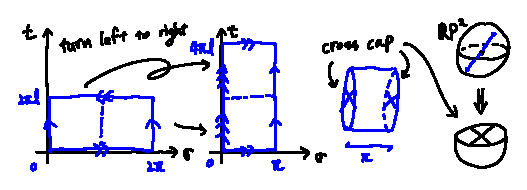
\includegraphics[width=350pt]{KleinBottle.eps}}
\caption{Klein bottle. It can be described by a cylinder with cross cap boundary on both ends.}
\label{KleinBottle.eps}
\end{figure}
it should be
\begin{align}
 A_{0,K} = \frac{1}{2} \int \frac{dl}{2l}
 \tr \left[ \Omega (-1)^F \frac{1}{2}(b_0+\ol b_0) \frac{1}{2}(c_0+\ol c_0) q^{L_0 +\ol L_0 -\frac{c}{12}} \right] \qquad (q=e^{-2\pi l}) \ ,
\end{align}
where the factor of $\frac{1}{2}$ is from the projection operator $\frac{1+\Omega}{2}$,
or you can also regard it as an additional gauge redundancy $w \to \ol w$.



One can rewrite the amplitude as follows.
\begin{align}
 A_{0,K} = \frac{1}{2} \int \frac{dl}{2l}
 \tr \left[ (-1)^F b_0 c_0 q^{2L_0  -\frac{c}{12}} \right] \ ,
\end{align}
where $c = c_\mathrm{mat} +c_\mathrm{gs} = 0$, and 
\begin{align}
 L_0 = \frac{\alpha'}{4} p^2 +\sum_{n=1}^\infty \left( \alpha_{-n}\cdot \alpha_{n} +n b_{-n} c_n +n c_{-n} b_n \right) -1 \ .
\end{align}
Thus, the result is
\begin{align}
 A_{0,K} &= \frac{iV_{26}}{(2\pi l_s)^{26}} \int \frac{dl}{4l} \frac{1}{l^{13} \eta(2il)^{24}} \ , \\
 &= 2^{13} \frac{iV_{26}}{(2\pi l_s)^{26}} \int \frac{ds}{4} \eta(is)^{-24} \ .
\end{align}




\noindent
\textbf{M\"obius strip amplitude}


Finally, let us consider a M\"obius strip for WS (see Fig.~\ref{MobiusStrip.eps}).
\begin{figure}[htb]
\centerline{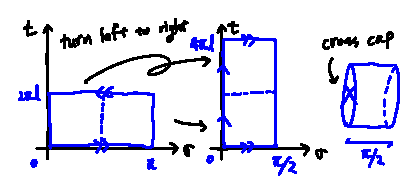
\includegraphics[width=300pt]{MobiusStrip.eps}}
\caption{M\"obius strip.}
\label{MobiusStrip.eps}
\end{figure}
It has
\vspace{-4pt}
\begin{itemize}
% \setlength{\parskip}{0cm}
 \setlength{\itemsep}{0pt}
 \item The range is $0 \le \sigma \le \pi$, the period is $2\pi l$, coming together with the orientation flip:
       $(t,\sigma) \sim (t+2\pi l,\pi -\sigma)$.
 \item There is a real modulus $l$; the amplitude needs a $b$ zero mode insertion.
 \item There is a real isometry, shift of $t$; the amplitude needs a $c$ zero mode insertion.
\end{itemize}

The M\"obius strip amplitude is
\begin{align}
 A_{0,M} = \frac{1}{2} \int \frac{dl}{2l}
 \tr \left[ \Omega (-1)^F b_0 c_0 q^{L_0 -\frac{c}{12}} \right] \qquad (q=e^{-2\pi l}) \ .
\end{align}
The trace is over Hilbert space of the matter and ghost sectors on the strip
as well as the Chan-Paton index, which gives in total $n^2$ degeneracy for each state.
We can divide the effect of $\Omega$ into two parts as follows.
\begin{align}
 \Omega |\Phi;\Lambda\rangle = |\Omega\Phi;P\Lambda^TP \rangle
 \equiv \Omega_\Phi \cdot \Omega_\Lambda |\Phi;\Lambda\rangle \ .
\end{align}
Let us see the $\Omega_\Lambda$, which is defined as
\begin{align}
 \Omega_\Lambda = \frac{P\Lambda^TP}{\Lambda} \ .
\end{align}
In the case of $SO(n)$, which means $P=1$,
\begin{align}
 \Omega_{\Lambda,SO} = \frac{\Lambda^T}{\Lambda} =
 \begin{cases}
  +1 \qquad (\textrm{for symmetric $\Lambda$})  \\
  -1 \qquad (\textrm{for anti-symmetric $\Lambda$})
 \end{cases} \ ,
\end{align}
Therefore,
\begin{align}
 \tr_{\Lambda,SO} \left[ \Omega \right] = \frac{n(n+1)}{2} -\frac{n(n-1)}{2} = n \ .
\end{align}
In the case of $Sp(n)$ (exercise)
\begin{align}
 \tr_{\Lambda,Sp} \left[ \Omega \right] = -n \ .
\end{align}
The matter and ghost part is
\begin{align}
 \tr_\Phi \left[ \Omega (-1)^F b_0 c_0 q^{L_0 -\frac{c}{12}} \right]
 &= \frac{iV_{26}}{(2\pi l_s)^{26}} \frac{1}{(2l)^{13}}
 \cdot q^{-1} \prod_{n=1}^\infty \frac{(1-(-q)^n)^2}{(1-(-q)^n)^{26}}  \nn
 &= \frac{iV_{26}}{(2\pi l_s)^{26}} \frac{1}{(2l)^{13}} \cdot \frac{-1}{\eta(il+\frac{1}{2})^{24}} \ .
\end{align}
Therefore, the M\"obius strim amplitude is
\begin{align}
 A_{0,M} &= \pm n \cdot \frac{iV_{26}}{(2\pi l_s)^{26}} \int \frac{dl}{4l}
 \frac{1}{(2l)^{13}} \cdot \frac{-1}{\eta(il+\frac{1}{2})^{24}} \ ,  \\
 &= \mp n \cdot \frac{iV_{26}}{(2\pi l_s)^{26}} \int \frac{ds}{2}
 \eta(is+\frac{1}{2})^{-24} \ ,
\end{align}
where we used $\sqrt{2l} \eta(il+\frac{1}{2}) = \eta(\frac{i}{4l}+\frac{1}{2})$.



To sum up, three amplitudes are
(introduced additional $\frac{1}{2}$ factor for Cylinder as an unoriented amplitude)
\begin{align}
 A_{0,C} &= \frac{n^2}{2^{13}} \cdot \frac{iV_{26}}{(2\pi l_s)^{26}}
 \int_0^\infty \frac{ds}{4} \eta(is)^{-24} \ ,  \\
 A_{0,K}
 &= 2^{13} \cdot \frac{iV_{26}}{(2\pi l_s)^{26}} \int \frac{ds}{4} \eta(is)^{-24} \ ,  \\
 A_{0,M}
 &= \mp 2n \cdot \frac{iV_{26}}{(2\pi l_s)^{26}} \int \frac{ds}{4}
 \eta(is+\frac{1}{2})^{-24} \ ,
\end{align}
where
\begin{align}
 &\eta(is)^{-24} = q^{-1} +24 +\mathcal O(q) \qquad (q = e^{-2\pi s}) \ ,  \\
 &\eta(is+\frac{1}{2})^{-24} = -q^{-1} +24 +\mathcal O(q) \ .
\end{align}
As we saw in oriented string case the massless states lead IR singularity.
On the other hand, in the unoriented open string case we have
\begin{align}
 \frac{1}{2^{13}} \left[ n\mp 2^{13} \right]^2 \cdot \frac{iV_{26}}{(2\pi l_s)^{26}}
 \int_0^\infty \frac{ds}{4} \cdot 24 \ ,
\end{align}
which vanish for $SO(2^{13}=8192)$.
This cancellation can be illustrated as like Fig.~\ref{tadpoleCancel.eps}.
\begin{figure}[htb]
\centerline{\includegraphics[width=250pt]{tadpoleCancel.eps}}
\caption{Pictorical expression for the unoriented open string amplitude.}
\label{tadpoleCancel.eps}
\end{figure}
The cross cap shows another object (other than D-brane) that absorb and emit
gravitons etc., which is called O-plane.
In this situation it should be space-filling, hence, it is O$25^\pm$-plane
($+$ for $Sp$ and $-$ for $SO$).
O$25^\pm$-plane has $\pm 2^{13}$ times that of D$25$-brane,
and so single O$25^-$-plane cancel tension of $2^{13}$ D$25$-branes.



Although our discussion was in bosonic string,
parallel argument perfectly works for superstring and it leads that
\textbf{the IR divergence vanishes for $SO(32)$}.
This means that
\begin{align}
 \textrm{Type I} = \textrm{Type IIB} +32 \textrm{ D$9$-branes} +\textrm{O$9^-$-plane} \ .
\end{align}
Note that in the superstring case D-branes and O-plane have RR-charge
in addition to tension, which has relations
\begin{align}
 T_{\mathrm{O}9^\pm} = \pm 32 \cdot T_{\mathrm{D}9} \quad (\textrm{tension}) \ , \quad
 Q_{\mathrm{O}9^\pm} = \pm 32 \cdot Q_{\mathrm{D}9} \quad (\textrm{RR-charge}) \ .
\end{align}






\subsection{T-duality of type I theory}


Let us recall T-duality.
Consider $X^{i}$ is $S^1$ compactified and T-duality acts as follows:
\begin{align}
 T_{i}:  \quad X^{i}(z,\ol z) = X^{i}(z) +\ol X^{i}(\ol z) \quad\to\quad
 X^{\prime i}(z,\ol z) = X^{i}(z) -\ol X^{i}(\ol z) \ .
\end{align}
On the other hand, the orientation flip acts as follows:
\begin{align}
 \Omega: \quad X^{i}(z,\ol z) = X^{i}(z) +\ol X^{i}(\ol z) \quad\to\quad
 X^{i}(\ol z,z) = \ol X^{i}(z) +X^{i}(\ol z) \ .
\end{align}
Therefore, in the T-dual coordinate $X'$ the orientation flip acts as
\begin{align}
 \Omega: \quad X^{\prime i}(z,\ol z) \quad\to\quad
 -X^{\prime i}(\ol z,z) \ .
\end{align}
This is understood as space-time \textbf{oribfold}
as well as world-sheet orientation flip (see Fig.~\ref{s1orbifold.eps}),
which is called \textbf{orientifold}.
\begin{figure}[htb]
\centerline{\includegraphics[width=100pt]{s1Orbifold.eps}}
\caption{$\ZZ_2$ orbifold of $S^1$.}
\label{s1orbifold.eps}
\end{figure}
Therefore, the dual space is not $S^1$ but $S^1/\ZZ_2$
with radius $\wt R = \frac{\alpha'}{R}$.
Note that there are two fixed points, where O-planes sit and
causes the ST reversal and the orientaiton flip.

Let us consider type I superstring theory with $X^9$ compactified on $S^1$
and take T-duality along the $S^1$.
With a proper Wilson line
\begin{align}
 A_9 = i
 \begin{pmatrix}
  & -a_1 & & & \\
  a_1 & & & & \\
  & & & -a_2 & \\
  & & a_2 & & \\
  & & & & \ddots
 \end{pmatrix}
\end{align}
D$8$-branes sit at different points in $\ZZ_2$ symmetric way (see Fig.~\ref{type1dual.eps}).
\begin{figure}[htb]
\centerline{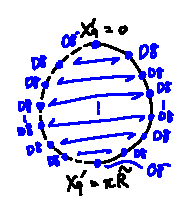
\includegraphics[width=100pt]{type1dual.eps}}
\caption{T-dual of type I superstring theory.}
\label{type1dual.eps}
\end{figure}
Note that an O$9^-$-plane splits into two O$8^-$-plane.
Accordingly, tension and RR-charge reduce by $2$.


In the end, T-dual of type I on $S^1$ is
\begin{align}
 \textrm{Type IIA on } S^1/\ZZ_2 \quad \textrm{with} \quad  2 \textrm{ O$8^-$-plane }
 + 32 \textrm{ D$8$-branes }.
\end{align}
Of course, one can consider further T-dualities along other directions.
Each T-duality doubles the number of O-planes, and hence,
reduces the tension and the RR-charges.
Namely, we have following relations:
\begin{align}
 T_{\mathrm{O}p^\pm} = \pm 2^{p-4} \cdot T_{\mathrm{D}p} \quad (\textrm{tension}) \ , \quad
 Q_{\mathrm{O}p^\pm} = \pm 2^{p-4} \cdot Q_{\mathrm{D}p} \quad (\textrm{RR-charge}) \ .
\end{align}






% \begin{thebibliography}{CDLOGP91}

%  \bibitem[Pol98]{Pol98}
%                 J. Polchinski.
%                 String theory. Vol. 1.
%                 Cambridge University Press, 1998.

%  \bibitem[BP09]{Blumenhagen:2009zz}
%                R.~Blumenhagen and E.~Plauschinn.
%                \newblock {Introduction to conformal field theory}.
%                \newblock {\em Lect. Notes Phys.}, 779:1--256, 2009.

% \end{thebibliography}


% \bibliography{string-lecture}
% \bibliographystyle{halpha}
% \bibliographystyle{JHEP}

% \begin{thebibliography}{CDLOGP91}

% %\cite{AlvarezGaume:1981hn}
% \bibitem[AFM81]{AlvarezGaume:1981hn}
%   L.~Alvarez-Gaume, D.~Z.~Freedman and S.~Mukhi,
%   ``The Background Field Method and the Ultraviolet Structure of the Supersymmetric Nonlinear Sigma Model,''
%   Annals Phys.\  {\bf 134}, 85 (1981).
%   %doi:10.1016/0003-4916(81)90006-3
%   %%CITATION = doi:10.1016/0003-4916(81)90006-3;%%
%   %525 citations counted in INSPIRE as of 09 Oct 2017



% \bibitem[CT88]{Callan:1988xx}
%  Curt Callan and Lárus Thorlacius.
%  \textit{SIGMA MODELS AND STRING THEORY.}
%  TASI Lecture, 1988.
%  (The link below is a direct link to the pdf file of 45MB )
%  \href{http://www.damtp.cam.ac.uk/user/tong/string/sigma.pdf}
%  {http://www.damtp.cam.ac.uk/user/tong/string/sigma.pdf}.




% \end{thebibliography}


\label{lastpage}

% \begin{tikzpicture}[>=stealth,scale=1]
%  \draw[->] (0,0)--(1,0);
%  \draw[latex-stealth] (0,0.5)--(1,0.5);
%  \draw[latex-stealthnew,arrowhead=2mm] (0,1)--(1,1);
% \end{tikzpicture}

% \begin{figure}[htb]
% \centerline{\includegraphics[width=250pt]{.eps}}
% \caption{}
% \label{.eps}
% \end{figure}



% \begin{table}[htbp]
%  \begin{center}
%   \caption{}
%   \vspace{4pt}
%   \label{table:001}
% \begin{tabular}{|c|c|c|c|c|}
% \hline
% \hline
%   Category & Sector & $(h_A,h_B,h_T)$ & Mirror theory & ABJM model \\
% \hline
%  1 & & \parbox{40pt}{$(0,0,0)$ $(1,1,1)$} & $1.11906$ & $1.13290$ \\
% \hline
%  2 & & \parbox{40pt}{$(0,0,1)$ $(1,1,0)$} & $-0.10861$ & $-0.10861$ \\
% \hline
%  \multirow{2}{*}{\vspace{-15pt}3} & 3-1 & \parbox{40pt}{$(0,1,0)$ $(1,0,1)$} & $0.176777$ &
%  \multirow{2}{*}{\vspace{-15pt}$0.176577$} \\
% \cline{2-4}
%  & 3-2 & \parbox{40pt}{$(1,0,0)$ $(0,1,1)$} & $0.176777$ & \\
% \hline
% \hline
% \end{tabular}
% \end{center}
% \end{table}


% \begin{thebibliography}{99}

% % \cite{Imamura:2012rq}
% \bibitem{Imamura:2012rq}
%   Y.~Imamura and D.~Yokoyama,
%   %``S^3/Z_n partition function and dualities,''
%   JHEP {\bf 1211}, 122 (2012)
%   [arXiv:1208.1404 [hep-th]].
%   %%CITATION = ARXIV:1208.1404;%%

 % \bibitem{fnorio:legendre}
 %         fnorio
 %         ``ルジャンドル変換とは何か''
 %         \url{http://fnorio.com/0146Legendre_transformation/Legendre_transformation.html}


 % \bibitem{EMAN:dynamics}
 %         EMAN物理学
 %         ``ハミルトニアン''
 %         \url{http://eman-physics.net/analytic/hamilton.html}


 % \bibitem{Wiki:legendre}
 %         Wiki
 %         ``ルジャンドル変換''
 %         \url{https://ja.wikipedia.org/wiki/ルジャンドル変換}

 % \bibitem{mathtrain:legendre}
 %         高校数学の美しい物語
 %         ``ルジャンドル変換の意味と具体例''
 %         \url{http://mathtrain.jp/legendrehenkan}

% \end{thebibliography}


% \bibliography{dd}

\end{document}
